\documentclass[tikz,border=12pt]{standalone}
\usepackage[T1]{fontenc}
\usepackage{mathpazo}
\usepackage{amsmath,amssymb}
\usetikzlibrary{arrows.meta, positioning, calc, fit}

\definecolor{stblue}{HTML}{7B97AD}
\definecolor{rwgold}{HTML}{B8995E}
\definecolor{sage}{HTML}{7A9A7E}
\definecolor{dkbrown}{HTML}{3D3530}
\definecolor{wmgray}{HTML}{7B7067}
\definecolor{cream}{HTML}{F9F6F0}
\definecolor{border}{HTML}{D4C9B8}
\definecolor{terracotta}{HTML}{C47A6A}
\definecolor{lavender}{HTML}{907EA0}

\begin{document}
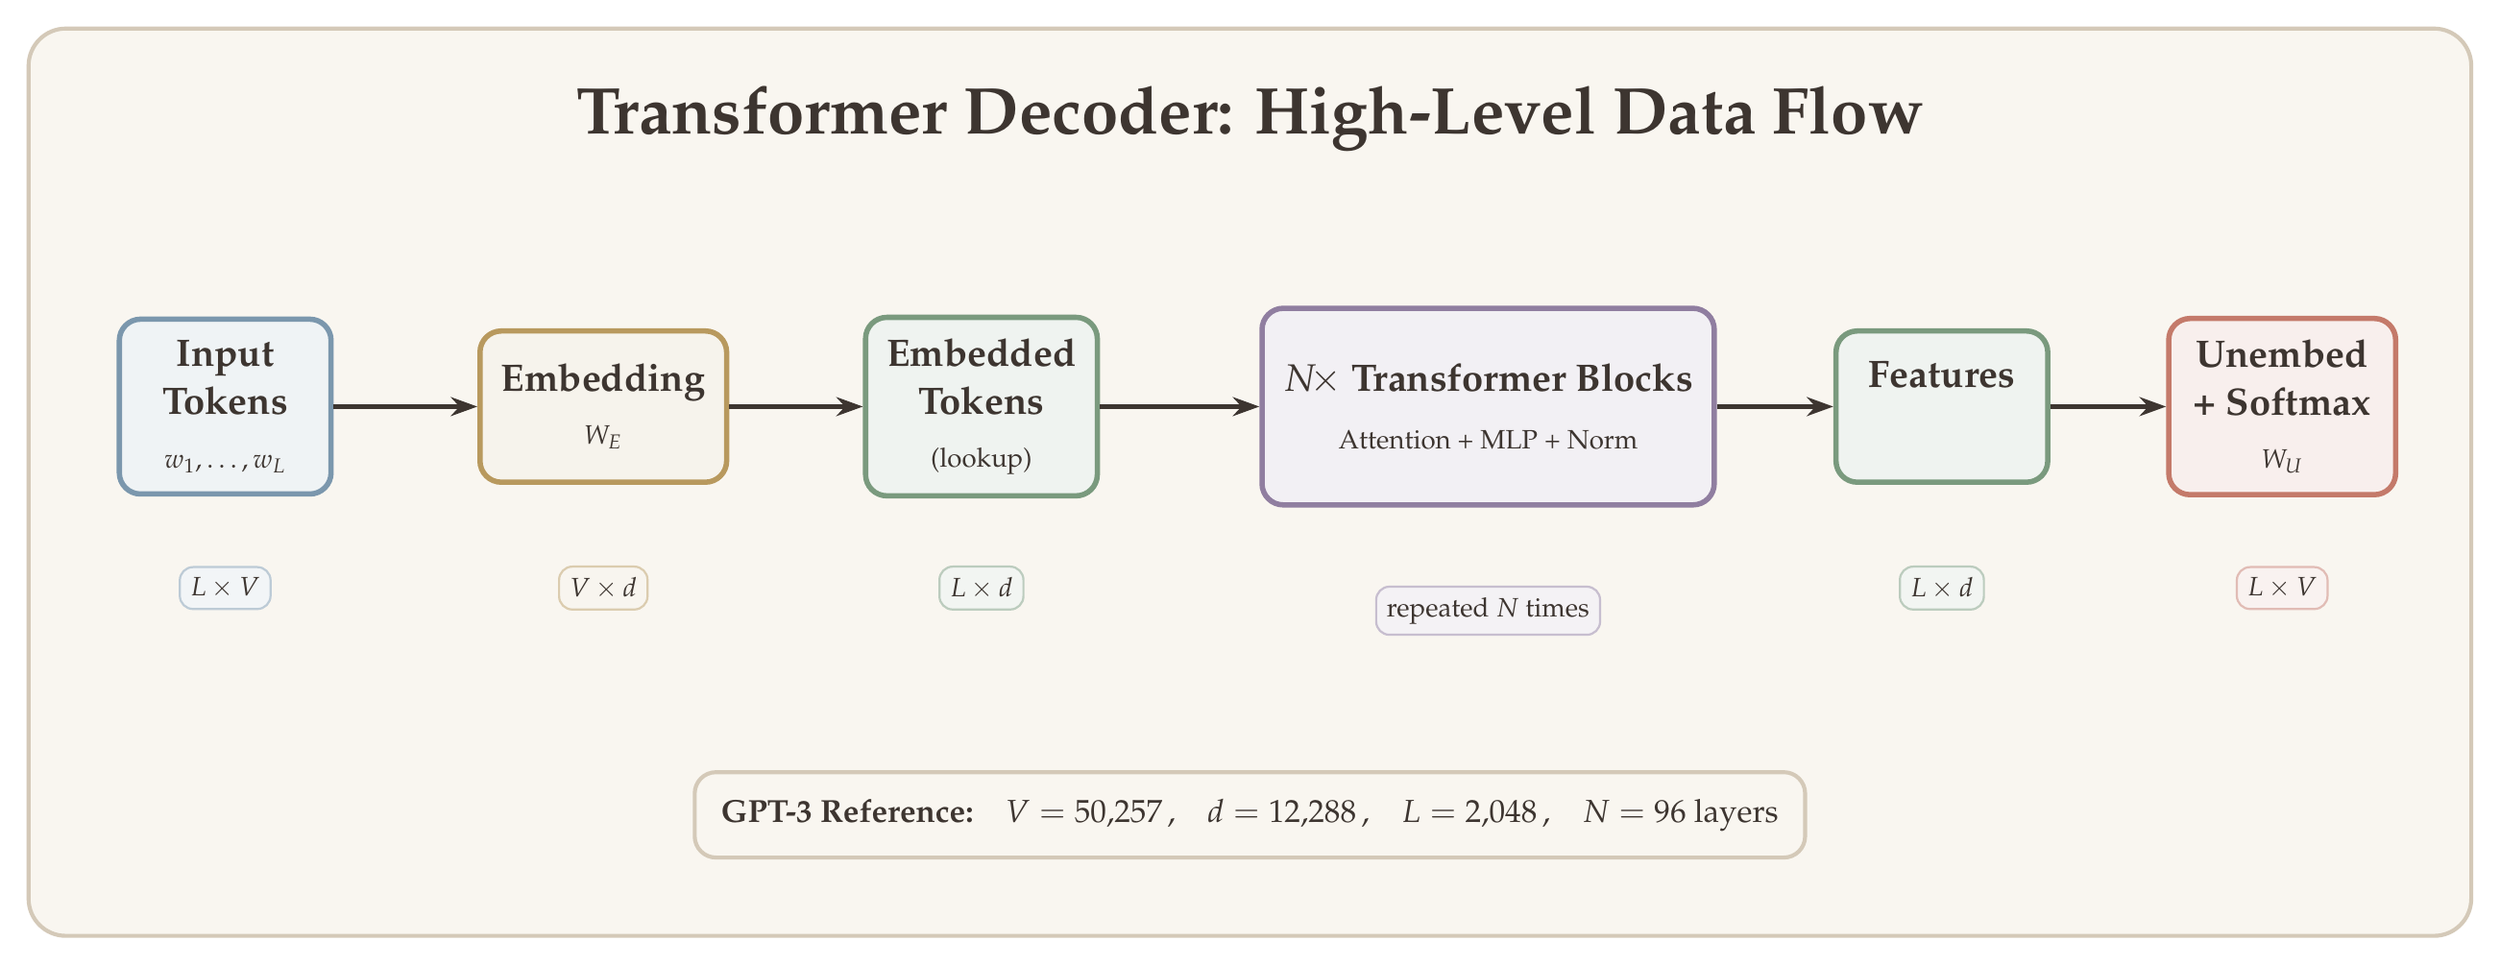
\begin{tikzpicture}[
  >={Stealth[length=3.5mm, width=2.5mm]},
  box/.style={
    draw=#1, line width=2pt, fill=#1!12, rounded corners=8pt,
    minimum height=20mm, font=\Large\bfseries, text=dkbrown,
    align=center, inner sep=8pt
  },
  dimbox/.style={
    rounded corners=5pt, fill=#1!10, draw=#1!50,
    line width=0.8pt, font=\normalsize, text=dkbrown,
    inner sep=4pt, align=center
  },
  arr/.style={->, line width=2pt, dkbrown},
]

% Background
\fill[cream, rounded corners=14pt] (-1.8,-5.8) rectangle (30.5,6.2);
\draw[border, rounded corners=14pt, line width=1.5pt] (-1.8,-5.8) rectangle (30.5,6.2);

% Title
\node[font=\Huge\bfseries, text=dkbrown] at (14.35,5.0)
  {Transformer Decoder: High-Level Data Flow};

% ===== Main flow nodes =====

% Input tokens
\node[box=stblue, minimum width=28mm] (input) at (0.8,1.2)
  {Input\\Tokens\\[2pt]
   {\normalsize\mdseries $w_1, \ldots, w_L$}};
\node[dimbox=stblue] at (0.8,-1.2) {$L \times V$};

% Embedding matrix
\node[box=rwgold, minimum width=28mm] (embed) at (5.8,1.2)
  {Embedding\\[2pt]
   {\normalsize\mdseries $W_E$}};
\node[dimbox=rwgold] at (5.8,-1.2) {$V \times d$};

% Embedded tokens
\node[box=sage, minimum width=28mm] (embedded) at (10.8,1.2)
  {Embedded\\Tokens\\[2pt]
   {\normalsize\mdseries (lookup)}};
\node[dimbox=sage] at (10.8,-1.2) {$L \times d$};

% Transformer blocks (large box)
\node[box=lavender, minimum width=48mm, minimum height=26mm] (transformer) at (17.5,1.2)
  {$N\!\times$ Transformer Blocks\\[4pt]
   {\normalsize\mdseries Attention + MLP + Norm}};
\node[dimbox=lavender] at (17.5,-1.5) {repeated $N$ times};

% Features
\node[box=sage, minimum width=28mm] (features) at (23.5,1.2)
  {Features\\[6pt]{}};
\node[dimbox=sage] at (23.5,-1.2) {$L \times d$};

% Unembedding + Softmax
\node[box=terracotta, minimum width=30mm] (unembed) at (28,1.2)
  {Unembed\\+ Softmax\\[2pt]
   {\normalsize\mdseries $W_U$}};
\node[dimbox=terracotta] at (28,-1.2) {$L \times V$};

% ===== Arrows =====
\draw[arr] (input.east) -- (embed.west);
\draw[arr] (embed.east) -- (embedded.west);
\draw[arr] (embedded.east) -- (transformer.west);
\draw[arr] (transformer.east) -- (features.west);
\draw[arr] (features.east) -- (unembed.west);

% ===== GPT-3 reference table =====
\node[draw=border, line width=1.5pt, fill=cream, rounded corners=8pt,
      inner sep=10pt, font=\large, text=dkbrown, align=left]
  at (14.35,-4.2)
  {\textbf{GPT-3 Reference:}\quad
   $V = 50{,}257$\,,\quad
   $d = 12{,}288$\,,\quad
   $L = 2{,}048$\,,\quad
   $N = 96$ layers};

\end{tikzpicture}
\end{document}
